%~~~~~~~~ Chapter ~~~~~~~~
\chapter{Quantum computing}
In this chapter we make a quick introduction to quantum computation \red{and stuff}
\section{What is a Qubit}
In classical computing the basic element of information is a known as a bit. All the information that we can think of in our computers is encoded in a set of bits.
For instance one of the most famous ways of encoding text is the so-called \ac{ascii} encoding, in this case we use 7 bits to encode all the letters and numbers and some symbols, for instance $a=1100001$, $A=10000011$, $b=1100010$, and so on.

Classical bits can only take two values, namely 0 or 1, $+$ or $-$, $\uaw$ or $\daw$, and all the operations that we do in our everyday lives is restricted to flip or not the states of some bits, from photograph editing, to music players, to web browsing, to the hardest scientific calculations, everything that requires a computer at the end of the day is just flipping the correct bits.

% Current processors operate on 64bits each time, taking into account that an standard computer operates at $\approx 2\cdot10^9 MHz$ it means that this can operate about $100\cdot10^9$ bits per second

There are many different types of bits. In early computers a bit would be a hole in a cardboard and its states would be the presence or absence of a hole. Later on it would be electrically controlled like an electrical switch, or a flip-flop circuit, or any other system with two different states that can be easily manipulated.

Recent computers use the magnetization of small cells as bits. This means that the physical representation of a bit of classical information nowadays is just a bunch of spins pointing in one direction or the other.

Even when spins are intrinsically quantum objects in current computers no intrinsically quantum property is exploited.


And here is where the Quantum bits appear. The qubit.


If we narrow down the physical representation of the information to the state of a quantum system with two states, what is commonly known as a \ac{2ls}, we could have the qubit in the $\ket{0}$ or $\ket{1}$ states as well as in any combination of them. Formally the state of a qubit could be expressed as
\begin{equation}
  \ket{\psi} = \cos\frac{\theta}{2}\ket{0} +e^{i\phi}\sin\frac{\theta}{2}\ket{1}
\label{genstate}
\end{equation}
If the chosen physical representation for the qubit would be a spin $S=1/2$ in the presence of a magnetic field, the geometrical interpretation of such an state shown in figure \ref{Bsph}. Nevertheless many physical implementations of qubits exist nowadays, so the interpretation of the general state is not universal.


Notice that as opposed to classical bits, a qubit can have a continuum\footnote{not really, precision, Heisenberg...} of states of states.

%~~~~~~~~~~~~~~~~~~~~~~~~~~ FIGURE ~~~~~~~~~~~~~~~~~~~~~~~~~%
\begin{figure}[!h]
\centering
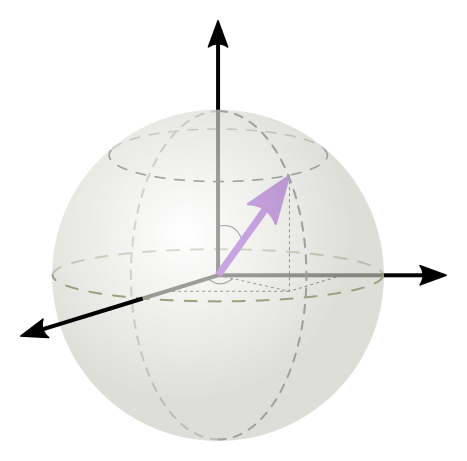
\includegraphics[width=0.5\textwidth]{chapter02/figures/bloch_sphere.png}
\vspace{-5pt}
\caption{Bloch sphere that represents all the possible states of a $S=1/2$ spin.}
\label{Bsph}
\end{figure}
\FloatBarrier
%~~~~~~~~~~~~~~~~~~~~~~~~~~~~~~~~~~~~~~~~~~~~~~~~~~~~~~~~~~~%

Nevertheless the idea of having qubits goes far beyond the possibility of storing more states per qubit\footnote{In fact probably quantum memories will not be such a great idea since they could be quite volatile}.

The great advantage that the quantum computation brings is that we can actually perform operations in combinations of these states. \red{finish}








\section{An example: the Deutsch's problem}
This problem is the simplest example where a quantum speed up is demonstrated\cite{Deutsch1992}. Even when the speed up is only a factor $\times2$ and the problem is purely academic, it contains all the ingredients to understand the essence of quantum computing.

The Deutsch's problem can be stated as follows:

\paragraph{Given an unkown black box that works as a binary 1 bit function $f(x)$, how can we know if it is a constant function, or a balanced function evaluating it only once?\\}
\textcolor{white}{.}\\
Notice that there are only 4 possible functions (see table \ref{binfunc}) that take one input with two possible states and returns one output with two possible states.
\begin{table}[h!]
\begin{center}
\begin{tabular}{c|c|c|c|c}
% \hline
\multicolumn{1}{l|}{Input} & \multicolumn{1}{l|}{$A$} & \multicolumn{1}{l|}{$B$} & \multicolumn{1}{l|}{$C$} & \multicolumn{1}{l}{$D$} \\ \hline
$\uaw$ & $\uaw$ & $\uaw$ & $\daw$ & $\daw$ \\ %\hline
$\daw$ & $\uaw$ & $\daw$ & $\uaw$ & $\daw$ \\ %\hline
% 0 & 0 & 0 & 1 & 1 \\ %\hline
% 1 & 0 & 1 & 0 & 1 \\ %\hline
\end{tabular}
\end{center}
\vspace{-15pt}\caption{The only four possible binary functions of 1 bit}
\label{binfunc}
\end{table}

On one hand we have the options $A$ and $D$ that always return either 0 or 1 regardless of the input, for this reason we will refer to them as constant functions.
On the other hand, $B$ and $C$ flips or not one of the states. In fact, using classical computation language, $B$ and $C$ perform the NOT function. We will refer to these options as balanced functions.\\

Classically to solve the Deutsch's problem (find if the black-box $f(x)$ is balanced or constant) we need to evaluate the function for both inputs.

If we meassure the input $\uaw$, and get $\uaw$: $f(\uaw)=\uaw$ the function could be either $A$ (constant) or $B$ (balanced), so we need to know the behavior of $f(\daw)$ to distinguish between these two possibilities.
There is no way around it. No matter how we address this problem, classically, we will always need to evaluate the function twice.

But quantum computation offers the resources to figure out the nature of the function $f(x)$ with only one evaluation. To understand how this works we just need to define two quantum gates.


\subsection{Two quantum gates}
To show how the Deutsch's problem can be tackled quantum-computationally we will need to understand a 1-qubit gate called the Hadamard gate, and a 2-qubit gate that acts like the (classical) controlled NOT gate.

The description of the gates (and the problem) will be done for a generic qubit with two states $\ket{\uaw}$ and $\ket{\daw}$.

\subsubsection{The Hadamard Gate}
The Hadamard gate acts on a single qubit by mapping the states as follows:
\begin{equation}
  \ket{\uaw} \longrightarrow \frac{\ket{\uaw}+\ket{\daw}}{\sqrt{2}}
  \quad\quad;\quad\quad
  \ket{\daw} \longrightarrow \frac{\ket{\uaw}-\ket{\daw}}{\sqrt{2}}
  % \ket{0} \longrightarrow \frac{\ket{0}+\ket{1}}{\sqrt{2}} \quad\quad;\quad\quad
  % \ket{1} \longrightarrow \frac{\ket{0}-\ket{1}}{\sqrt{2}}
\label{Hmap}
\end{equation}
The matrix representation (in the basis $\mathcal{B}=\left\{\ket{\uaw},\ket{\daw}\right\}$) is:
% The matrix representation (in the basis $\mathcal{B}=\left\{\ket{0},\ket{1}\right\}$) is:
\begin{equation}
  H=\frac{1}{\sqrt{2}}\left(\begin{array}{cc}
  1 & 1 \\
  1 & -1
  \end{array}\right)
\label{hadamard}
\end{equation}
Notices that this gate is an unitary operation: $H\cdot H^{\dagger}=\mathbb{I}$.

To understand what this gate means physically it is useful to imagine our qubit as an spin $1/2$ particle in the presence of a magnetic field.
In this physical representation the Hadamard gate would correspond to switching on a magnetic field along the $X$ direction for a certain time so the state initially in the $\pm1_z$ state would evolve to the $\pm1_x$ state.

In other physical implementation this gate would require a different physical process, but its action needs to be the mapping described in \eqref{Hmap}.


\subsubsection{The CNOT Gate}
The other gate that we need is the CNOT gate. This is a 2-qubit function that flips the second qubit state only if the first qubit is in the state $1$. For describing the state of the two qubits we need an slightly more complex basis:
\begin{equation}
  \mathcal{B}=
  \left\{\ket{\uaw;\uaw},\ket{\uaw;\daw},\ket{\daw;\uaw},\ket{\daw;\daw}\right\}
  % \mathcal{B}=\left\{\ket{0_10_2},\ket{0_11_2},\ket{1_10_2},\ket{1_11_2}\right\}
\end{equation}
\red{Modify notation} In this notation the subindex $1,2$ refers to the qubit, and the value $0,1$ refers to the state of the corresponding qubit that are chosen to be the eigenvectors of the $S_z$ operator.
In this basis the CNOT gate would be expressed:
\begin{equation}
  \text{CNOT}=\left(\begin{array}{cc|cc}
  1 & 0 & 0 & 0 \\
  0 & 1 & 0 & 0 \\\hline
  0 & 0 & 0 & 1 \\
  0 & 0 & 1 & 0
  \end{array}\right)
\end{equation}
Notice that this gates %XXX (as all the gates)
is also unitary, meaning that $\text{CNOT}\cdot\text{CNOT}^{\dagger}=\mathbb{I}$


If we think again in the spin $1/2$ particle in a magnetic field as the physical representation this function would be the process of measuring the first qubit state and applying a magnetic field in the $X$ only if the state of the first qubit is $+1$

The mapping that this function performs in our basis vectors is the following:
\begin{equation}
  \begin{split}
    &\ket{\uaw;\uaw}\rightarrow\ket{\uaw;\uaw} \quad\quad;\quad\quad
    \ket{\uaw;\daw}\rightarrow\ket{\uaw;\daw}\\
    &\ket{\daw;\uaw}\rightarrow\ket{\daw;\daw} \quad\quad;\quad\quad
    \ket{\daw;\daw}\rightarrow\ket{\daw;\uaw}
    % &\ket{0_10_2}\rightarrow\ket{0_10_2} \quad\quad;\quad\quad
    % \ket{0_11_2}\rightarrow\ket{0_11_2}\\
    % &\ket{1_10_2}\rightarrow\ket{1_11_2} \quad\quad;\quad\quad
    % \ket{1_11_2}\rightarrow\ket{1_10_2}
  \end{split}
\end{equation}
Since we are using the eigenvectors of each qubit as building blocks for our basis, all the states can be expressed as product states\blue{rephrase}. Expressing the previous mapping in these terms will be useful later on.
Any state of the basis $\ket{\phi_i}$ can be expressed as direct product of the the state of the first qubit $\ket{x}$ and the state of the second qubit $\ket{y}$, this is  $\ket{\phi_i}=\ket{x}\otimes\ket{y}$.
Using this notation, the mapping for the CNOT function can be written as follows:

\begin{equation}
  \begin{array}{lcl}
    \ket{x} & \longrightarrow & \ket{x} \\
    \ket{y} & \longrightarrow & \ket{x\oplus y}
  \end{array}
\end{equation}
this means that the CNOT gate is equivalent to apply a \ac{xOr}\footnote{The XOR gate (2 bits for the input) is a controlled NOT gate (1 bit input) that reverses the second qubit only if the control bit takes value $\daw$.} controlled by the first qubit. It is useful to remember that XORding any input with 0 ($\uaw$) returns the same input while XORding any input with 1 ($\daw$) returns the opposite input, denoted by a tilde.
\begin{equation}
  \uaw\oplus y = y \quad\quad;\quad\quad \daw\oplus y = \tilde{y}
\end{equation}

With these two gates we are ready to address the Deutsch's problem using quantum computation.

\subsection{The Deutsch's Problem}
The formal proposal of the Deutsch's problem\footnote{the original problem deals with a function $f:\{ 0,1\}^n\rightarrow\{ 0,1\}$, but the simplest case, $n=1$, is enough to understand all the ingredients needed for quantum computation} is the following:\\

We are given a black box quantum computer known as an oracle that implements some function $f:\{ 0,1\}\rightarrow\{ 0,1\}$, this is, it takes n-digit binary values as input and produces either a 0 or a 1 as output for each such value. We are promised that the function is either constant (0 on all inputs or 1 on all inputs) or balanced (returns 1 for half of the input domain and 0 for the other half); the task then is to determine if $f$ is constant or balanced by using the oracle as few times as possible. \\

This means that there would be a quantum speed-up if we could distinguish whether
\begin{equation}
  f(\uaw) = f(\daw) \quad\quad \text{or}\quad\quad f(\uaw) = \tilde{f}(\daw)
  % f(0) = f(1) \quad\quad \text{or}\quad\quad f(0) = \tilde{f}(1)
  \label{problem}
\end{equation}
evaluating the funcion $f(x)$ only once.\\

This is in fact possible by using two qubits $x$, $y$, and some quantum gates. The complete scheme can be seen in figure \ref{fcnot}.
%~~~~~~~~~~~~~~~~~~~~~~~~~~ FIGURE ~~~~~~~~~~~~~~~~~~~~~~~~~%
\begin{figure}[!h]
  \centering
  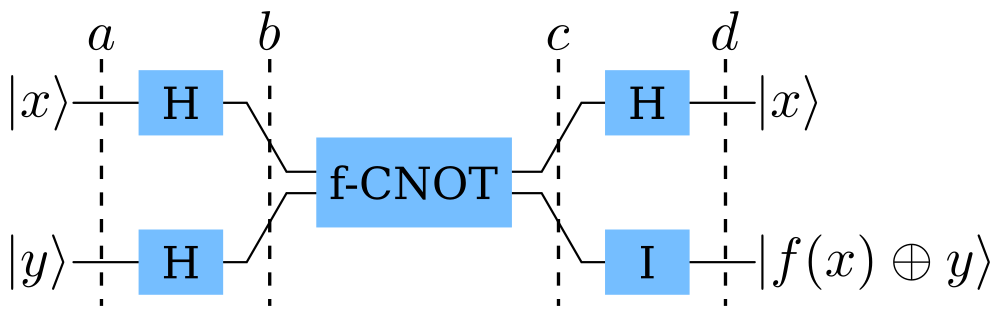
\includegraphics{chapter02/figures/fcnot.png}
  \vspace{-5pt}
  \caption{Scheme of the system used for solving the Deutsch's problem. The H boxes represent Hadamard gates, and the I box is am identity gate. The different stages of the algorithm are marked by letters a,b,c,d.}
  \label{fcnot}
\end{figure}
\FloatBarrier
%~~~~~~~~~~~~~~~~~~~~~~~~~~~~~~~~~~~~~~~~~~~~~~~~~~~~~~~~~~~%
As stated before, classically we would need to evaluate the oracle $f(x)$ twice, while using a quantum computer we would only need to do it once. To  do so we will use a modified CNOT gate such that one of the input bits is evaluated by the $f$ function. This can be expressed as follows
\begin{equation}
  \begin{array}{lcl}
    \ket{x} & \longrightarrow & \ket{x} \\
    \ket{y} & \longrightarrow & \ket{f(x)\oplus y}
  \end{array}
  \label{fCNOT}
\end{equation}
Notice that this modified CNOT gate (fCNOT) only evaluates the function on one of the qubits, $f(x)$.\\


In the initial state (stage $a$) we will have both qubits in the same state. We will use the following notation:
\begin{equation}
  \ket{\psi_{a}} = \ket{\uaw;\uaw} \quad\quad\text{or equivalently}\quad\quad
  \ket{x}=\uaw\text{, }\ket{y}=\uaw
  % \ket{\psi_{a}} = \ket{1_11_2} \quad\quad;\quad\quad (\ket{x}=1, \ket{y}=1)
\end{equation}
We run each qubit through a Hadamard gate, eq \eqref{hadamard}, so the state at the stage $b$ would be:
\begin{equation}
  \ket{\psi_{b}} =
  \left(\frac{\ket{\uaw}-\ket{\daw}}{\sqrt{2}}\right)\otimes
  \left(\frac{\ket{\uaw}-\ket{\daw}}{\sqrt{2}}\right) =
  \frac{1}{2}\left(\ket{\uaw;\uaw}-\ket{\uaw;\daw}-
  \ket{\daw;\uaw}+\ket{\daw;\daw}\right)
  % \ket{\psi_{b}} =
  %  \left(\frac{\ket{0_1}-\ket{1_1}}{\sqrt{2}}\right)\otimes
  %  \left(\frac{\ket{0_2}-\ket{1_2}}{\sqrt{2}}\right) =
  % \frac{1}{2}\left(\ket{0_10_2}-\ket{0_11_2}-
  %                  \ket{1_10_2}+\ket{1_11_2}\right)
\end{equation}
Notice that this state $\ket{\psi_b}$ is a \textbf{non-entangled superposition of all the possible inputs}, so by just one evaluation of the $f(x)$ function we would be calculating all the possible outputs simultaneously.

This is where the great advantage of the quantum computation becomes apparent since it allows the simultaneous evaluation of many different inputs as a superposition of them.

When we feed the state $\ket{\psi_b}$ to the f-CNOT gate we would get the following state at the stage $c$
\begin{equation}
  \ket{\psi_{c}} = \frac{1}{2}
  \left(\ket{\uaw;f(\uaw)} - \ket{\daw;f(\daw)} - \ket{\uaw;\tilde{f}(\uaw)}+
  \ket{\daw;\tilde{f}(\daw)} \right)
  % \ket{\psi_{c}} = \frac{1}{2}
  % \left(\ket{0_1f(0_1)_2} - \ket{1_1f(1_1)_2} - \ket{0_1\tilde{f}(0_1)_2}+
  % \ket{1_1\tilde{f}(1_1)_2} \right)
\end{equation}
In case this is not clear, let's do the explicit calculation. Using the shortcut \eqref{fCNOT}
For the first two terms:
\begin{equation}
  \begin{split}
    \text{f-CNOT}\ket{\uaw;\uaw} &=
    \ket{\uaw}\otimes\ket{f(\uaw)\oplus\uaw} =\ket{\uaw;f(\uaw)}\\
    \text{f-CNOT}\ket{\daw;\uaw} &=
    \ket{\daw}\otimes\ket{f(\daw)\oplus \uaw} = \ket{\daw;f(\daw)}
    % \text{f-CNOT}\ket{0_10_2} &=
    %  \ket{0_1}\otimes\ket{f(0_1)\oplus 0_2} =  \ket{0_1 f(0_1)_2}\\
    % \text{f-CNOT}\ket{1_10_2} &=
    %  \ket{1_1}\otimes\ket{f(1_1)\oplus 0_2} = \ket{1_1 f(1_1)_2}
  \end{split}
\end{equation}
Notice that the evaluation of $f(x)$ is now XORded with 0 ($\uaw$), coming from the first qubit, so the second qubit should not be modified.
In case the notation gets messy let's point out that $\ket{\daw;f(\daw)}$ will be either $\ket{\daw;\uaw}$ or $\ket{\daw;\daw}$, depending on the behavior of $f(x)$.

The calculation for the last two terms yields:
\begin{equation}
  \begin{split}
    \text{f-CNOT}\ket{\uaw;\daw} &=
    \ket{\uaw}\otimes\ket{f(\uaw)\oplus \daw} = \ket{\uaw;\tilde{f}(\uaw)}\\
    \text{f-CNOT}\ket{\daw;\daw} &=
    \ket{\daw}\otimes\ket{f(\daw)\oplus \daw} = \ket{\daw;\tilde{f}(\daw)}
    % \text{f-CNOT}\ket{0_11_2} &=
    %  \ket{0_1}\otimes\ket{f(0_1)\oplus 1_2} = \ket{0_1\tilde{f}(0_1)_2}\\
    % \text{f-CNOT}\ket{1_11_2} &=
    %  \ket{1_1}\otimes\ket{f(1_1)\oplus 1_2} = \ket{1_1\tilde{f}(1_1)_2}
  \end{split}
\end{equation}
Notice that the evaluation of $f(x)$ is now XORded with 1 ($\daw$), hence it will be flipped.\\

Now, depending on the unknown nature of $f(x)$, eq \eqref{problem}, we could rewrite $\ket{\psi_c}$ in two different ways.
\begin{equation}
  \begin{split}
    &\text{if f is constant:   }f(\uaw)=f(\daw)\quad\Rightarrow\quad
    \ket{\psi_c}=
    \frac{1}{2}(\ket{\uaw}-\ket{\daw})\otimes
    (\ket{f(\uaw)}-\ket{\tilde{f}(\uaw)})\\
    &\text{if f is balanced:   } f(\uaw)=\tilde{f}(\daw)\quad\Rightarrow\quad
    \ket{\psi_c}=
    \frac{1}{2}(\ket{\uaw}+\ket{\daw})\otimes
    (\ket{f(\uaw)}-\ket{\tilde{f}(\uaw)}) \\
    % &\text{if f is constant:   }f(0)=f(1)\quad\Rightarrow\quad
    % \ket{\psi_c}=
    % \frac{1}{2}(\ket{0_1}-\ket{1_1})\otimes
    %            (\ket{f(0_1)_2}-\ket{\tilde{f}(0_1)_2})\\
    % &\text{if f is balanced:   } f(0)=\tilde{f}(1)\quad\Rightarrow\quad
    % \ket{\psi_c}=
    % \frac{1}{2}(\ket{0_1}+\ket{1_1})\otimes
    %            (\ket{f(0_1)_2}-\ket{\tilde{f}(0_1)_2}) \\
  \end{split}
\end{equation}


Notice that the state of the first qubit ($\uaw$ or $\daw$) depends on whether the function $f(x)$ is constant or balanced, so just by running the state of the first qubit through a Hadamard gate we can know the nature of the function $f$:
\begin{equation}
  \begin{split}
    &\text{if f is constant:   }f(\uaw)=f(\daw)\quad\Rightarrow\quad
    \ket{\psi_d}= \ket{\daw}\otimes(\ket{f(\uaw)}-\ket{\tilde{f}(\uaw)})\\
    &\text{if f is balanced:   } f(\uaw)=\tilde{f}(\daw)\quad\Rightarrow\quad
    \ket{\psi_d}= \ket{\uaw}\otimes(\ket{f(\uaw)}-\ket{\tilde{f}(\uaw)})
    % &\text{if f is constant:   }f(0)=f(1)\quad\Rightarrow\quad
    % \ket{\psi_d}= \ket{1_1}\otimes(\ket{f(0_1)_2}-\ket{\tilde{f}(0_1)_2})\\
    % &\text{if f is balanced:   } f(0)=\tilde{f}(1)\quad\Rightarrow\quad
    % \ket{\psi_d}= \ket{0_1}\otimes(\ket{f(0_1)_2}-\ket{\tilde{f}(0_1)_2})
  \end{split}
\end{equation}

If the final state of the first qubit after the whole process is $\ket{\daw}$, then we know that $f(x)$ is a constant function whereas if the final state is $\ket{\uaw}$ we know that $f(x)$ is balanced.\\

The main point in this example is that the function $f(x)$ \textbf{was executed only once, but it was executed on a superposition state containing all the possible inputs}.\\

Naturally this is the simplest example possible, and it only provides a $\times2$ speed up in a (not really relevant) problem. Nevertheless these concepts can be applied to many other algorithms allowing a huge speed up in very important problems such as factoring big numbers, critical for current encryption systems (Shor's algorithm, that runs in polynomial time) or searching in databases, important in unsupervised machine learning algorithms (Grover's algorithm $\mathcal{O}(n)\rightarrow\mathcal{O}(\sqrt{n})$)

\red{quantum chemistry, Quantum simmulations and stuff, proteins...}.

%~~~~~~~~~~~~~~~~~~~~~~~~~~ FIGURE ~~~~~~~~~~~~~~~~~~~~~~~~~%
\begin{figure}[!h]
  \centering
  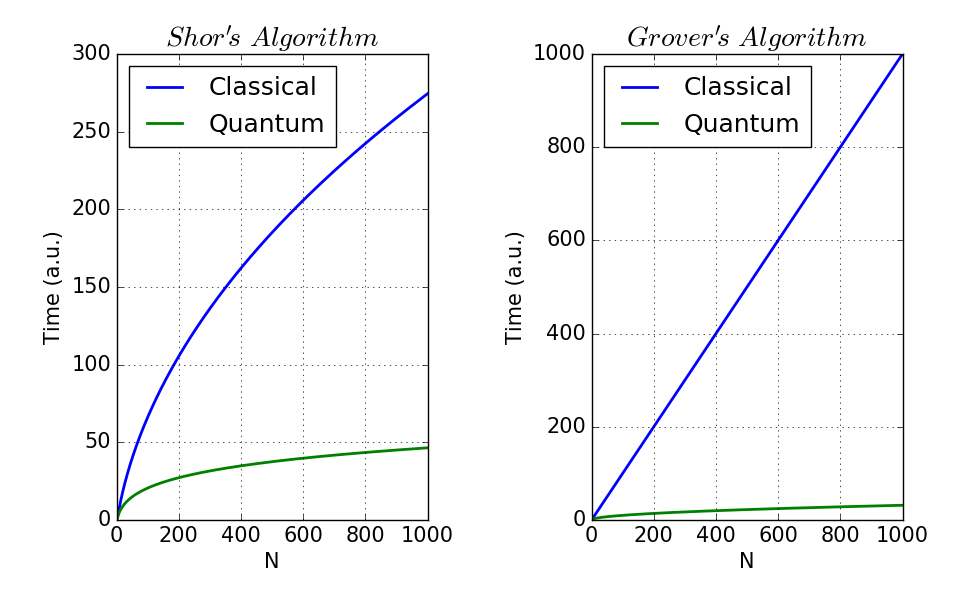
\includegraphics{chapter02/figures/quantum_scaling.png}
  \vspace{-5pt}
  \caption{Time order of the Shor and Grover's algorithm. Here we plot the scaling of the analogue classical algorithms (the best scaling we know so far) and the order of the quantum algorithm. Quantum computers allow a drastic change in the scaling of these algorithms.}
\end{figure}
\FloatBarrier
%~~~~~~~~~~~~~~~~~~~~~~~~~~~~~~~~~~~~~~~~~~~~~~~~~~~~~~~~~~~%
